%%%%%%%%%%%%%%%%%%%%%%%%%%%%%%%%%%%%%%%%%%%

% formato FRONTE RETRO
\documentclass[epsfig,a4paper,11pt,titlepage,twoside,openany]{book}
\usepackage{epsfig}
\usepackage{plain}
\usepackage{setspace}
\usepackage[paperheight=29.7cm,paperwidth=21cm,outer=1.5cm,inner=2.5cm,top=2cm,bottom=2cm]{geometry} % per definizione layout
\usepackage{titlesec} % per formato custom dei titoli dei capitoli

\singlespacing

\usepackage[italian]{babel}

%%%%%%%%%%%%%%%%% STEFANO ADDED %%%%%%%%%%%%%%%%
% supporto lettere accentate
% queste due righe nel preambolo servono a poter utilizzare le lettere accentate in tutto il testo se no di norma si inserirebbero con \'e...
\usepackage[T1]{fontenc}
\usepackage[utf8]{inputenc}
\usepackage{hyperref} %Serve per i riferimenti
\usepackage{caption}  %Serve per le note (caption)
\usepackage{multicol}	 %Serve per usare più colonne

%%%%%%%%%%%%%%%%% ENRICO ADDED %%%%%%%%%%%%%%%%%
\usepackage{ulem} %Serve per il sottolineato
\usepackage{amsmath} %Serve per alcuni ambienti matematici
\usepackage{array} %Serve per le tabelle
\usepackage{multirow} %Seve per tabelle
\setcounter{secnumdepth}{5} %Utilissimo serve per aumentare il numero di paragrafi, si arriva fino a 5 livelli di profondità x.x.x.x.x
%GRAFICI
\usepackage{pgfplots}
\usepackage{pgfmath}
\usepackage{tikz}
%CODICE
% \usepackage{listings}
% \usepackage[cache=false]{minted} 
%\setminted{tabsize=4, breaklines, breakanywhere, linenos, mathescape,}

% \lstset{
% 	  breakatwhitespace=false,         
% 	  breaklines=true,     
% 	  basicstyle=\footnotesize\ttfamily,            
% 	  commentstyle=\color{blue}, %Indica il colore dei commenti
% 	  keywordstyle=\color{red}, %Indica il colore delle parole chiave
% 	  language=C, %Indica il linguaggio predefinito da usare
% 	  rulecolor=\color{black}, %Indica il colore dei numeri di righe
% 	  tabsize=4,
% 	  escapeinside={\%*}{*)},
% 	  morekeywords={}, %Altre parole da inserire tra le keywords. Ad esempio possiamo aggiungere do, gotttto, ecc ecc 
% }
%%%%%%%%%%%%%%%%% END OF ENRICO  %%%%%%%%%%%%%%%%

\begin{document}
%set the language of the text to italian
% !TeX spellcheck = it_IT

%%%%%%% personal commands (ALIAS):
% \newcommand{\nome_commando}[argomenti]{comando}
\newcommand{\e}[1]{$\cdot 10^{#1}$}
\newcommand{\mmax}[0]{mod\_withMax }
\newcommand{\mover}[0]{mod\_overlap }
\newcommand{\mmod}[0]{modularità modificata }
\newcommand{\nv}[0]{Node2Vec }
\newcommand{\wv}[0]{Word2Vec }
\newcommand{\cnrl}[0]{CNRL }
\newcommand{\cora}[0]{Cora }
\newcommand{\citeseer}[0]{Citeseer }
\newcommand{\LPred}[0]{Link Prediction }
%



%
\chapter{Esperimenti}
\section{Origini dei grafi}
In questa sezione vengono spiegati i dataset utilizzati e le loro origini.\\
Si possono dividere in due gruppi, non solo perché tali gruppi al loro interno presentino caratteristiche d'affinità, ma anche in quanto i grafi che vi appartengono sono stati utilizzati nel corso del tirocinio per due applicazioni differenti. Nella Tabella~\ref{tab:dati_grafi} sono elencati i dettagli tecnici di ogni dataset.
%
\begin{center}
	\begin{tabular}{|l|r|r|r|c|c|r|}
		\hline
		grafi&nodi&archi&archi/nodi&diretto&etichette&attributi\\
		\hline
		Cora & 2708 & 5429 & 2.0 & sì & 7 & 1433\\
		Citeseer & 3312 & 4732 & 1.4 & sì & 6 & 3703\\
		\hline
		BlogCatalog & 10312 & 333983 & 32.4 & no & 39 & 0\\
		Gnutella & 6301 & 20777 & 3.3 & no & 0 & 0\\
		Dolphins & 62 & 159 & 2.6 & no & 0 & 0\\
		Karate & 35 & 78 & 2.2 & no & 0 & 0\\
		\hline
		\end{tabular}
		\captionof{table}{Per ogni grafo sono indicate le sue caratteristiche principali}
		\label{tab:dati_grafi}
\end{center}
%
\subsection*{Esperimento principale: Cora - Citeseer}\cite{Co-Ci_1}\cite{Co-Ci_2}
Il dataset di \textbf{Cora} è un grafo diretto che rappresenta una rete di articoli scientifici sull'apprendimento automatico, ogni nodo è un articolo. Mentre ogni arco rappresenta il collegamento fra un documento è l'altro, se il documento $A$ cita il documento $B$ si avrà l'arco $(A, B)$. La rete è costruita in modo che ogni nodo abbia almeno un arco entrante o uscente.\\
Ogni articolo appartiene ad esattamente una classe identificata da un etichetta. Ogni attributo rappresenta la presenza (deve apparire almeno 10 volte) o meno di una determinata parola nel testo del documento.\\
\\
Il dataset di \textbf{Citeseer} è un grafo diretto che rappresenta una rete analoga a quella di Cora, anche qui si hanno articoli scientifici che si citano vicendevolmente. L'etichetta è la classe d'appartenenza cui l'articolo appartiene, e gli attributi son nuovamente la presenza o meno di certe parole nel testo.\\
%
\subsection*{Grafi per esperimenti minori}
Questi quattro grafi vengono presentati in ordine decrescente nel numero dei nodi, così come fatto nella seconda parte della Tabella~\ref{tab:dati_grafi}.\\
\begin{itemize}
	\item \textbf{BlogCatalog}\cite{BlogCatalog} rappresenta la rete di relazioni, di conoscenza, fra gli utenti di alcune piattaforme per blog
	\item \textbf{Gnutella}\cite{Gnutella_1}\cite{Gnutella_2} questo grafo si rifà alla rete peer-to-peer per lo scambio di file di Gnutella nell'agosto 2002. Ogni nodo rappresenta un host e ogni arco un collegamento fra due host
	\item \textbf{Soc-Dolphins}\cite{Dolphins_1}\cite{Dolphins_2} riporta la rete sociale di un gruppo di delfini al largo della Nuova Zelanda nel 2003
	\item \textbf{Karate}\cite{Karate} raccoglie lo storico degli incontri in un club di karate universitario nel 1977. Ogni nodo è un membro del club, ogni arco indica uno scontro terminato in pareggio
\end{itemize}
%
\section{Modello di un grafo}
In questa sezione viene spiegato cosa si intende per modello di un grafo, e perché è tanto importante per gli algoritmi che vi sono costruiti sopra.\\
Come descritto nel capitolo sull'implementazione è necessario visitare il grafo per generare su di questo dei cammini. Questi vengono presi in input dall'algoritmo di \wv che tramite una rete neurale va a descrivere ogni nodo che s'individua tramite un vettore di valori reali, mentre \cnrl utilizza un metodo alternativo chiamato Latent Dirichlet Allocation (LDA)\cite{LDA} o una sua variante detta HalfLDA.\\
\begin{figure}[htp]
	\centering
	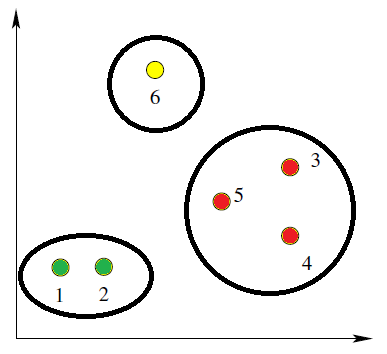
\includegraphics{immagini/punti_modello}
	\caption{Son visualizzati i nodi d'un grafo che vengono rappresentati da un modello che dispone di due dimensioni}
	\label{fig:grafico_modello}
\end{figure}
\\
\begin{center}
	\begin{tabular}{|l|cc|}
		\hline
		ID&X1&X2\\
		\hline
		1 & 1 & 2\\
		2 & 2 & 2\\
		3 & 7 & 5\\
		4 & 7 & 3\\
		5 & 5 & 4\\
		6 & 3 & 8\\
		\hline
	\end{tabular}
	\captionof{table}{Tabella rappresentativa del modello dei nodi in Figura~\ref{fig:grafico_modello}}
	\label{tab:coordinate_modello}
\end{center}
Di norma ogni vettore è lungo $64$, e ogni numero reale rappresenta una posizione lungo un asse in un piano a $64$ dimensioni. Si può però pensare anche ad un caso più semplice, ad esempio in Figura~\ref{fig:grafico_modello} si possono vedere sei punti che si può immaginare appartenessero ad un grafo e fossero legati fra loro in qualche modo. Una volta che son stati generati i cammini su tale grafo, e questi forniti ad uno dei due algoritmi, viene ritornata la Tabella~\ref{tab:coordinate_modello} dove ad ogni ID di un nodo vengono associati due valori (qui interi per semplicità), sono usati due valori perché così son facili da mostrare con $64$ sarebbe pressoché impossibile. Si possono dunque immaginare come coordinate su un piano cartesiano, ed è così che si arriva alla Figura~\ref{fig:grafico_modello}, qui visivamente si può dire che esistono 3 gruppi distinti che sono evidenziati dai colori, abbiamo quindi $(1, 2) - (3, 4, 5) - (6)$.\\
Escludendo l'influenza dei colori, il nostro occhio ci suggerisce l'esistenza di questi 3 gruppi in quanto i nodi che vi fanno parte sono vicini fra loro, questo è esattamente ciò che ci si aspetta dalla definizione di somiglianza, tanto più due nodi sono vicini tanto più questi sono simili. Si ricorda che esistono comunque molte definizioni formali di somiglianza e la distanza euclidea è solo una di queste.\\
\\
Di conseguenza se due nodi molto simili, e quindi vicini, vengono collegati da un arco allora tale arco assume un valore molto elevato, vicino a $1$, diversamente assumerà un valore molto basso, vicino a $0$, se i nodi che lega sono diversi ossia molto lontani, questo valore lo chiameremo da ora in avanti coerenza\footnote{è il nome migliore che m'è venuto in mente non c'è un vero e proprio termine tecnico per questa definizione} di un arco.
%
\section{Link Prediction}
Ecco il primo di tre algoritmi, che verranno spiegati in questo capitolo, tutti si basano sul modello del grafo appena spiegato.\\
L'algoritmo di \LPred ha lo scopo d'assegnare un valore al grafo in input, questo valore è una percentuale e per tale motivo ricade nell'intervallo $[0, 1]$. Questa percentuale sta a rappresentare la coerenza degli archi del grafo, nel dettaglio un arco è molto coerente se lega due nodi simili, un grafo è tanto più coerente tanti più archi coerenti ha.
%
\subsection{Dinamiche di funzionamento}
Per primo viene caricato il grafo, sempre come lista d'archi in quanto sono questi il fulcro dell'algoritmo. Si va a spezzare gli archi in due gruppi dopo averli mescolati per non creare delle divisioni sempre uguali, tale rottura viene fatta sulla base del parametro $F$ che indica quale sarà la percentuale degli archi adibiti all'addestramento del modello e quali invece saranno adibiti alla fase di test.\\
Il numero degli archi usati per il test viene dato dalla Formula~\ref{eq:n_archi_fake}
\begin{equation}
	m \cdot \frac{1}{F}
	\label{eq:n_archi_fake}
\end{equation} 
\begin{equation}
	m \cdot \left( 1- \frac{1}{F} \right)
	\label{eq:n_archi_true}
\end{equation}
mentre quelli utilizzati per l'addestramento corrispondono alla Formula~\ref{eq:n_archi_true}, dove $m$ è il numero di archi del grafo.\\
Il nuovo grafo (\textbf{G1}) creatosi, inseguito alla rimozione degli archi per il test, viene utilizzato per generare il modello.\\
Per ogni arco appartenente all'insieme di test (\textbf{Test=T}) se ne genera un altro (\textbf{Check=C}) tramite una coppia di nodi casuali assicurandosi che non corrispondano ad un arco già esistente. Si hanno quindi tre insiemi, il primo adibito all'addestramento stabilisce il modello necessario a discernere quale dei due restanti è la migliore selezione.
Per ogni arco, di T e C, si va a veder quanto sono simili i nodi che lega e se ne calcola così la coerenza, grazie all'apposita funzione di similarità, ora disponibile. Gli archi possono essere valutati sulla base di questo nuovo parametro.\\
Siamo interessati a capire quanto erano buoni gli archi originari del grafo, T, rispetto a quelli generati casualmente, C. 
\begin{equation}
	\frac{\left( n_1 + \frac{n_2}{2} \right)}{n}
	\label{eq:AUC_formula}
\end{equation}
Si usa perciò la metrica detta AUC\cite{AUC_metric}, che si basa sulla Formula~\ref{eq:AUC_formula}, dove gli elementi sono:
\begin{itemize}
	\item $n$ è il numero di archi presenti nell'insieme di test, calcolato mediante la Formula~\ref{eq:n_archi_fake}
	\item $n1$ sono le volte in cui un arco di test T è migliore di un arco casuale di C
	\item $n2$ sono le volte in cui un arco di test T ha pari valore o quasi rispetto ad un arco casuale di C
\end{itemize}
Per ogni arco di T se ne associa casualmente un altro di C, e qui si guarda quanto valgono i due archi coinvolti se l'arco di T vale più dell'arco di C si incrementa di $1$ il valore di AUC se uguali o quasi si incrementa di $0.5$. Avendo fatto ciò con ogni arco se ne calcola la media.\\
\\
Il valore finale della metrica AUC dipende fortemente da quale metodo si adotta per abbinare gli archi appartenenti a T e C, un accoppiamento sbagliato può fortemente sbilanciare il risultato, è per questo motivo che si va ad utilizzare un abbinamento casuale.\\
Inoltre si ha il parametro $F$ che influisce infatti più questo si avvicina a $1$ più cresce il numero di archi da utilizzare per la fase di test, diminuiscono di conseguenza i dati su cui fare affidamento per creare un buon modello che rappresenti appieno il grafo di partenza, e quindi il valore finale da aspettarsi è tendenzialmente più basso.\\
È necessario ricordare che la stima qui calcolata dipende fortemente dalla selezione iniziale, ed è per questo motivo che tutto questo processo non viene svolto solo una volta bensì $F$ volte, così da andare a stabilizzare il valore calcolato tramite la media di tutte le iterazioni. Inoltre questo permette di utilizzare via via tutti gli archi per addestrare il modello di \textbf{G1}.\\
\\
L'intero algoritmo si basa su confrontare gli archi grazie al valore che li rappresenta per individuare i più rilevanti, e quindi la parte più importante e critica è la generazione di tale valore mediante la funzione di similarità.\\
Questa può essere definita in tante maniere differenti in quanto si possono pesare diversi aspetti. Un esempio classico è basato sulla distanza euclidea più due nodi sono distanti nella rappresentazione del modello meno sono simili. Verranno mostrate le applicazioni di altre funzioni di similarità basate su diversi principi che però non verranno qui riportati.
%
\subsection{Esempio}
\begin{center}
	\begin{tabular}{|c|c|c|c|}
		\hline
		arco & autentico & dist & AUC\\
		\hline
		3-4 & sì & $2$ & \multirow{2}{*}{$1$}\\
		2-6 & no & $\sqrt{37}$ & \\
		\hline
		4-5 & sì & $\sqrt{5}$ & \multirow{2}{*}{$0.5$}\\
		3-5 & no & $\sqrt{5}$ & \\
		\hline
		5-6 & sì & $\sqrt{20}$ & \multirow{2}{*}{$0$}\\
		2-5 & no & $\sqrt{13}$ & \\
		\hline
		1-2 & sì & $1$ & \multirow{2}{*}{$1$}\\
		1-3 & no & $\sqrt{45}$ & \\
		\hline
	\end{tabular}
	\captionof{table}{Tabella riassuntiva del procedimento di \LPred}
	\label{tab:dati_es_prediction}
\end{center}
Consideriamo il modello descritto tramite la Figura~\ref{fig:grafico_modello} e la Tabella~\ref{tab:coordinate_modello}. Inoltre sappiamo che $F=2$, gli archi originali adibiti al test sono $(1, 2), (3, 4), (4, 5), (5, 6)$ mentre quelli generati casualmente sono $(3, 5), (2, 5), (2, 6), (1, 3)$, i due insiemi sono nello stesso numero per creazione e perché così possono essere confrontati.\\
Nelle prime due colonne della Tabella~\ref{tab:dati_es_prediction} sono riassunti gli archi e la loro origine. Le colonne seguenti rappresentano invece i passaggi successivi dell'algoritmo.\\
Nella terza colonna si può notare che ad ogni arco è stato associato un valore che rappresenta la distanza euclidea misurata sul piano cartesiano generato dal modello fra i due estremi dell'arco. Qui la funzione di similarità premia i valori più bassi a discapito degli altri. Inoltre la tabella è stata ordinata in modo che tutti gli archi di un insieme siano associati con uno dell'altro in maniera casuale, si può notare  infatti che nella seconda colonna "sì" e "no" si alternano.\\
Nell'ultima colonna viene rappresentato l'incremento che si andrà ad apportare alla metrica AUC grazie alla valutazione dei due archi corrispondenti. Questo valore dovrà poi esser diviso per il numero delle coppie in gioco per riportarlo nell'intervallo $[0, 1]$, in questo caso risulta $\displaystyle \frac{\left( 1+0.5+0+1 \right)}{4} = 0.625$\\
Si possono osservare alcuni peculiarità:
\begin{itemize}
	\item l'accoppiamento degli archi viene fatto in maniera casuale per evitare uno sbilanciamento
	\item una selezione a favore degli archi autentici porterebbe ad avere un incremento nullo del valore di AUC, al contrario si potrebbe avere un incremento di due unità se si favorissero  gli archi generati casualmente
	\item non si hanno archi ripetuti perché viene impedito alla creazione ma nulla vieta che un arco di C, corrisponda ad un arco usato in principio per generare il modello
	\item si può immaginare che più il valore di $F$ è grande e quindi più è grande la selezione di archi per l'addestramento (grazie alla Formula~\ref{eq:n_archi_true}) più il valore della calcolato cresca
\end{itemize}
L'algoritmo prevederebbe una seconda iterazione di tutto questo procedimento utilizzando gli archi in principio scartati come nuova base per il modello per poi calcolare la media delle percentuali.\\ Omettiamo questa fase perché uguale a quella appena illustrata.
%
\subsection{Risultati}
Le similarità utilizzate in questi esempi sono\cite{all_metric}:
\begin{itemize}
	\item DW = DeepWalk
	\item CN = Common Neighbors\cite{CN_metric}
	\item Salton = Salton Index\cite{Salton_metric}
	\item Jaccard = Jaccard Index
	\item RA = Resource Allocation\cite{RA_metric}
\end{itemize}
%
\begin{figure}[htp]
	\centering
	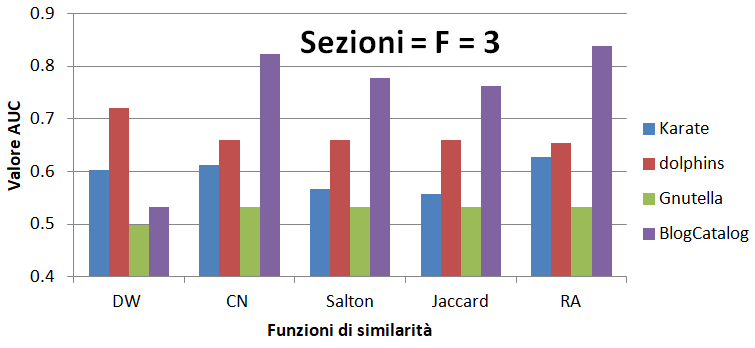
\includegraphics[width=\linewidth]{immagini/LP_fold3}
	\caption{\LPred con tre sezioni, $F=3$}
	\label{fig:LP_fold3}
\end{figure}
%
\begin{figure}[htp]
	\centering
	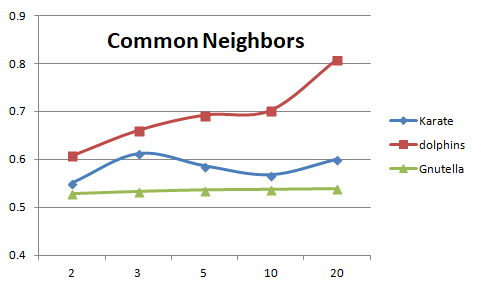
\includegraphics[width=\linewidth]{immagini/LP_CN}
	\caption{L'andamento della metrica di Common Neighbors, su tre grafi distinti attraverso differenti percentuali di selezione}
	\label{fig:LP_CN}
\end{figure}
%
\begin{figure}[htp]
	\centering
	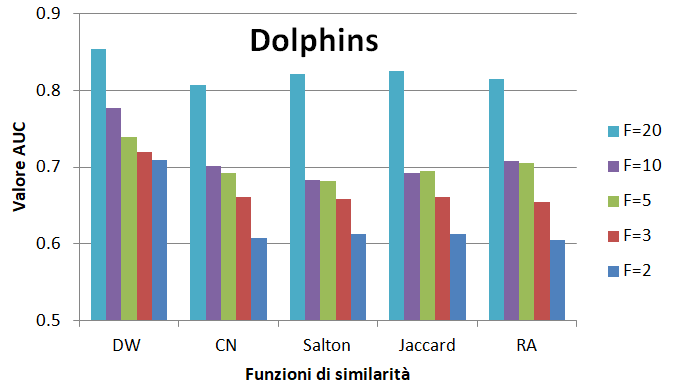
\includegraphics[width=\linewidth]{immagini/LP_Dolphins}
	\caption{L'andamento del grafo dolphins su diverse metriche attraverso differenti percentuali di selezione}
	\label{fig:LP_Dolphins}
\end{figure}
%
Questo algoritmo ha tre possibili variabili su cui si può lavorare:
\begin{itemize}
	\item \textbf{Il parametro $F$} (dall'inglese fold) che viene bloccato nella Figura~\ref{fig:LP_fold3}, si può notare come ogni grafo abbia un livello su cui si attesta, BlogCatalog grazie al fatto che è molto denso ha un valore in media molto alto rispetto ai tre grafi restanti
	\item Nella Figura~\ref{fig:LP_CN} si lavora su un \textbf{unica metrica}, si utilizza solo la funzione di similarità denominata Common Neighbors, che si basa sui nodi geometricamente vicini agli estremi di un arco all'interno del modello del grafo per valutare la somiglianza.\\
	Qui si può notare come all'aumentare del parametro $F$ il valore che si associa ad ogni grafo tende ad aumentare, questo è dovuto ad un modello meglio addestrato perché dispone di più dati in partenza, e quindi si ha una migliore valutazione
	\item La Figura~\ref{fig:LP_Dolphins} è forse la più semplice da osservare in quanto si osserva \textbf{un solo grafo}. Qui come prima si osserva che l'influenza del parametro $F$ è altissima sul risultato finale, inoltre si può vedere che le prestazioni di DeepWalk siano un attimo più alte rispetto al resto che invece tende ad avere le stesse performance 
\end{itemize}
Si precisa che questi sono degli esempi rappresentativi dell'andamento generale, che però non viene riportato in quanto sarebbe molto complesso da comprendere.
%
\section{Classificazione dei nodi}
Il problema della classificazione dei nodi/vertici punta a riconoscere partendo dalla rappresentazione di un elemento a quale classe questo appartiene, per definizione un elemento può appartenere ad una ed una sola classe, è tuttavia possibile pensare a classi interne ad altre classi o a sovrapposizioni. Per esempio data la classe A e la classe B si ha che, per come sono state definite, tutti gli elementi di A appartengono anche a B ($\displaystyle A \subseteq B$) di conseguenza $\displaystyle A \cap B = A$, tuttavia questo vale per l'insiemistica, nei problemi di classificazione fra A e B non c'è nessuna relazione e conseguentemente si ha che $\displaystyle A \cap B = \emptyset$.%esempio anche per intersezione???
%
\subsection{Dinamiche di funzionamento}
Il punto di partenza è costante, dato il grafo lo si visita per generare i cammini e con questi s'invoca l'algoritmo che genera il modello. Il modello viene disordinato e spezzato secondo il parametro di training ratio $T_r$, ossia percentuale d'addestramento, questo indica che percentuale del modello dovrà essere usata per l'addestramento, la restante sarà per i test.\\
In aggiunta si considerano anche le etichette o classi d'appartenenza di ogni nodo, si hanno quindi delle triplette contenenti:
\begin{itemize}
	\item ID del nodo che può anche essere dimenticato
	\item il vettore di numeri reali presi dal modello che lo rappresenta
	\item l'identificativo della classe a cui si appartiene
\end{itemize}
Con questi dati viene addestrata la funzione di classificazione, o classificatore, il cui scopo sarà predire la classe d'appartenenza dato in input il vettore di un qualche nodo.\\
\\
In seguito per ogni nodo appartenente all'insieme di test si cerca di predire la sua classe sottoponendo il suo vettore al classificatore e una volta terminato si confronta se l'esito corrisponde con la reale classe, nota grazie allo stesso file di etichette utilizzato per l'addestramento.\\
È importante far notare che il modello viene spezzato in due perché il classificatore deve essere addestrato su dati diversi da quelli che prenderà in seguito in input, altrimenti non ci sarebbe nulla da predire in quanto i dati passati vengono ricordati e quindi è impossibile sbagliare a dare una risposta.\\
\\
La valutazione delle predizioni effettuate può avvenire mediante il metodo più semplice ossia il \textbf{tasso d'errore}, che corrisponde alla Formula~\ref{eq:tasso_errore}, si contano quanti errori si son fatti rispetto al totale o si usa il metodo opposto ossia \textbf{l'accuratezza}, definita nella Formula~\ref{eq:accuratezza}, che conta i risultati con esito positivo rispetto al totale.
%
\begin{equation}
	T_{err} = \frac{N(errori)}{N(previsioni)}
	\label{eq:tasso_errore}
\end{equation}
%
\begin{equation}
	Acc = 1 - \left( \frac{N(errori)}{N(previsioni)} \right) = \frac{N(corretti)}{N(previsioni)}
	\label{eq:accuratezza}
\end{equation}
%
Se si vogliono fare delle misurazioni particolari si sfrutta invece la \textbf{matrice di confusione}, mostrata in Tabella~\ref{tab:matrice_confusione}, ideata inizialmente per valutare casi con solo due opzioni (Sì-positivo / No-negativo), può essere generalizzata per gestire la valutazione di un classificatore con più di due esiti, tramite due metodi differenti.
\begin{itemize}
	\item si amplia la matrice per avere invece che due righe e due colonne, K righe e colonne.\\
	Dove K è il numero di possibili valori ritornati dal classificatore
	\item si possono creare K matrici di confusione e ogni volta si sceglie una specifica classe come positiva tutte le altre vengono implose nel valore negativo
\end{itemize}
%
\begin{multicols}{2}
\begin{center}
	\begin{tabular}{cc|c|c| c|r|l|}
		 &  & \multicolumn{2}{|c|}{Previsione}\\
		 &  & Sì & No\\
		 \hline
		 Risposta & Sì & TP & FN\\
		 \hline
		 corretta & No & FP & TN\\
		\hline
	\end{tabular}
	\captionof{table}{Viene rappresentata una matrice di confusione}
	\label{tab:matrice_confusione}
	%
	\begin{tabular}{|c|c|}
		\hline
		TP & True Positive \\
		FN & False Negative \\
		FP & False Positive \\
		TN & True Negative \\
		\hline
	\end{tabular}
	\label{tab:MC_significato}
	\captionof{table}{Significato delle sigle della matrice di confusione}
\end{center}
\end{multicols}
%
Da questa matrice possiamo estrarre diverse misure:
\begin{itemize}
	\item \textbf{accuratezza} qui prende una nuova formulazione: $\displaystyle Acc = \frac{TP + TN}{TP + TN + FP + FN} $
	\item \textbf{sensibilità} penalizza le risposte negative sbagliate di conseguenza è meglio dare per positivo un esito se non è certo.\\
	Definita come: $\displaystyle S = \frac{TP}{TP + FN} $
	\item \textbf{precisione} penalizza le risposte positive sbagliate di conseguenza è meglio dare per negativo un esito se non è certo.\\
	Definita come: $\displaystyle P = \frac{TP}{TP + FP} $
	\item \textbf{Macro} precisione/sensibilità è la media aritmetica fra più valori di S o di P.\\
	Definita come: $\displaystyle Macro_{S} = \frac{S_1 + ... + S_n}{n} $
	\item \textbf{Micro} precisione/sensibilità è la media aritmetica delle componenti di S o di P prima di calcolarle, per poi considerarle un unica S o P.\\
	Definita come: $\displaystyle Micro_{P} = \frac{TP_1 + ... + TP_n }{ (TP_1 + ... + TP_n) + (FP_1 + ... + FP_n) } $
	\item \textbf{F1-Score} è la media armonica di: micro o macro o normale sensibilità e precisione.\\
	Definita come: $\displaystyle F1-Score = \frac{2}{ \frac{1}{S} + \frac{1}{P} } = \frac{2 \cdot S \cdot P}{ S + P }$
\end{itemize}
Nel nostro caso sensibilità e precisione non possono essere utilizzate in quanto ci sono troppi dati, mentre usare micro e macro non ha senso in quanto le classi sono perfettamente equivalenti, di conseguenza premiarne una a discapito di un'altra non ha significato. Per questo se serve si adotta l'F1-score. Tuttavia questa procedura non è veloce da calcolare pertanto spesso si adotta il più semplice e veloce metodo dell'accuratezza.
%
\subsection{Esempio}
\begin{center}
	\begin{tabular}{|c|c|c|c|c|}
		\hline
		ID & x & Previsione & Classe & Corretta\\
		\hline
		$5$ & $9$ & $0$ & $1$ & $0$\\
		$1$ & $13$ & $0$ & $0$ & $1$\\
		$2$ & $15$ & $0$ & $0$ & $1$\\
		$3$ & $27$ & $0$ & $1$ & $0$\\
		$4$ & $34$ & $1$ & $1$ & $1$\\
		$8$ & $36$ & $1$ & $0$ & $0$\\
		$6$ & $48$ & $2$ & $2$ & $1$\\
		$7$ & $59$ & $2$ & $2$ & $1$\\
		\hline
	\end{tabular}
	\captionof{table}{Tabella riassuntiva del procedimento di classificazione dei vertici}
	\label{tab:dati_es_classify}
\end{center}
Tutti i dati dell'esempio sull'algoritmo di classificazione sono riassunti nella Tabella~\ref{tab:dati_es_classify}. Nella prima colonna abbiamo gli ID dei nodi coinvolti, elemento che l'algoritmo ignora completamente, la seconda colonna contiene il vettore rappresentativo di ogni nodo, qui per semplicità è stato ridotto ad un solo numero.
%
\begin{equation}
	C(x)=
		\begin{cases}
			\begin{array}{ll}
				0 & se \ x < 30\\
				1 & se \ 30 \leq x \ \&\  x < 45\\
				2 & se \ 45 \leq x
			\end{array}
		\end{cases}
	\label{eq:classificatore_esempio}
\end{equation}
%
Si assume il classificatore definito nella Formula~\ref{eq:classificatore_esempio}, che darà come risposte i valori contenuti nella colonna "Previsione".\\
Mentre nella colonna "Classe" mostra il valore autentico del nodo. Infine nell'ultima colonna è indicato se la previsione è risultata corretta o meno.\\
\\
Per una valutazione mediante accuratezza è sufficiente calcolare la media aritmetica dell'ultima colonna, ossia $\displaystyle Acc = \frac{1+1+1+1+1}{8} = \frac{5}{8} = 0.625$. Mentre per l'F1-score sarebbe necessario calcolare sensibilità e precisione di ognuna delle 3 classi, riassumerli mediante micro o macro, ed infine arrivare ad un valore con F1-score.
%
\subsection{Risultati}
I grafi scelti per questa applicazione sono Cora (Figura~\ref{fig:VC_cora}) e Citeseer (Figura~\ref{fig:VC_citeseer}) perché fra quelli presentati nella Tabella~\ref{tab:dati_grafi} sono gli unici che sono forniti di attributi sui nodi, e questo permette di mostrare come l'utilizzo del grafo bipartito per l'introduzione degli attributi modifica le prestazioni.
%
\begin{figure}[htp]
	\centering
	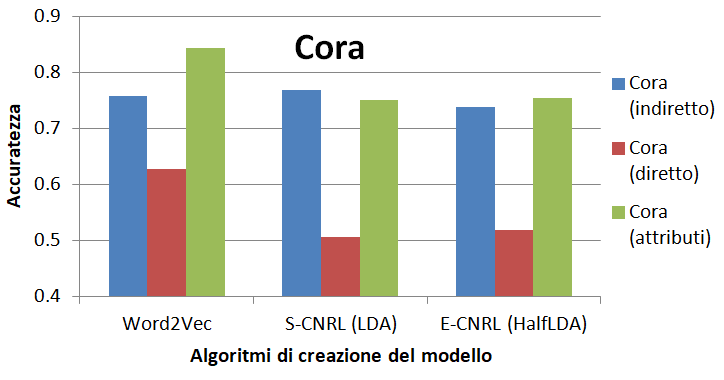
\includegraphics[width=\linewidth]{immagini/VC_cora}
	\caption{L'andamento del grafo Cora, con 3 differenti algoritmi di creazione del modello e 3 diverse interpretazioni iniziali, valutato mediante l'accuratezza}
	\label{fig:VC_cora}
\end{figure}
%
\begin{figure}[htp]
	\centering
	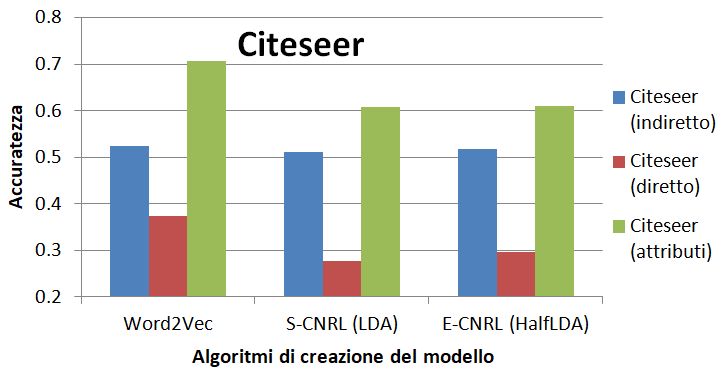
\includegraphics[width=\linewidth]{immagini/VC_citeseer}
	\caption{L'andamento del grafo Citeseer, con 3 differenti algoritmi di creazione del modello e 3 diverse interpretazioni iniziali, valutato mediante l'accuratezza}
	\label{fig:VC_citeseer}
\end{figure}
%
Sull'asse delle ordinate vi sono i valori compresi nell'intervallo $[0, 1]$ misurati mediante la tecnica dell'accuratezza. Mentre sull'asse delle ascisse vi sono i tre algoritmi utilizzati per creare il modello del grafo partendo dai cammini. \wv è il metodo di controllo, mentre S-CNRL e E-CNRL che lavorano rispettivamente con LDA e HalfLDA, sono i nuovi algoritmi proposti. Entrambi per alcune parti continuano ad usare \wv.\\
Sia Cora che Citeseer sono grafi originariamente diretti (misurazioni rosse), tuttavia si è provato ad interpretarli anche come se fossero indiretti (campionamento blu), l'ultimo andamento è dato dall'introduzione degli attributi (dati verdi).\\
Ecco alcuni dettagli che emergono dai due grafici:
\begin{itemize}
	\item \wv mostra prestazioni, anche se di poco, maggiori delle due alternative che invece tendono ad equivalersi
	\item la media dei valori delle misurazione nel grafico di Cora~\ref{fig:VC_cora} ($0.696$) rispetto a quella di Citeseer~\ref{fig:VC_citeseer} ($0.491$) è maggiore di circa $\displaystyle \frac{2}{10}$ questo è dovuto anche al fatto che Cora abbia una $\displaystyle densita' = \frac{archi}{nodi}$ maggiore rispetto a Citeseer
	\item un alta densità degli archi permette di creare molte interazioni fra i nodi e quindi il modello meglio rappresenta il grafo, si noti però che questo non è sempre facile da individuare, qui è presente uno stacco evidente in quanto entrambi i grafi hanno un estremamente bassa densità si dice infatti che sono sparsi
	\item si è provato ad aumentare la densità considerando ambo i grafi come indiretti (ogni arco indiretto può essere rappresentato come due archi diretti) si ha quindi poco meno di un raddoppio della densità, è infatti possibile che un arco avesse già il suo opposto e quindi non risente del cambiamento.
	L'effetto per entrambi è stato un innalzamento del valore medio lungo i 3 algoritmi usati
	\item con il grafo indiretto l'incremento di S-CNRL e E-CNRL è molto maggiore rispetto a quello di \wv questo può indicare, che \wv lavora molto bene con i grafi orientati a dispetto degli altri metodi
	\item l'introduzione degli attributi tramite il grafo bipartito ha notevolmente cambiato la situazione portando ad un incremento di prestazioni. Questi valori vanno confrontati con i dati del grafo orientato in quanto quello è il valore corretto, i punti blu del grafo non-orientato non sono comparabili in quanto servivano a mostrare come la densità influiva sul risultato tuttavia rappresentano un nuovo grafo diverso dall'originale, e quindi non paragonabile
\end{itemize}
%
\section{Valutazione dell'individuazione di comunità}

\end{document}